% ---------
% Preamble.
% ---------

% document type
\documentclass{article}

% import custom style
\usepackage{../.preamble/tikz_diagrams_template}

% color theme (black, red, blue, green, orange, purple, gold)
\colortheme{blue}

% ---------
% Document.
% ---------

\begin{document}

    % -----------------
    % TikZ environment.
    % -----------------

    \begin{tikzpicture}

        % -----------------
        % Airplane drawing.
        % -----------------
        
        \node[anchor=south west,inner sep=0] (image) at (0,0) {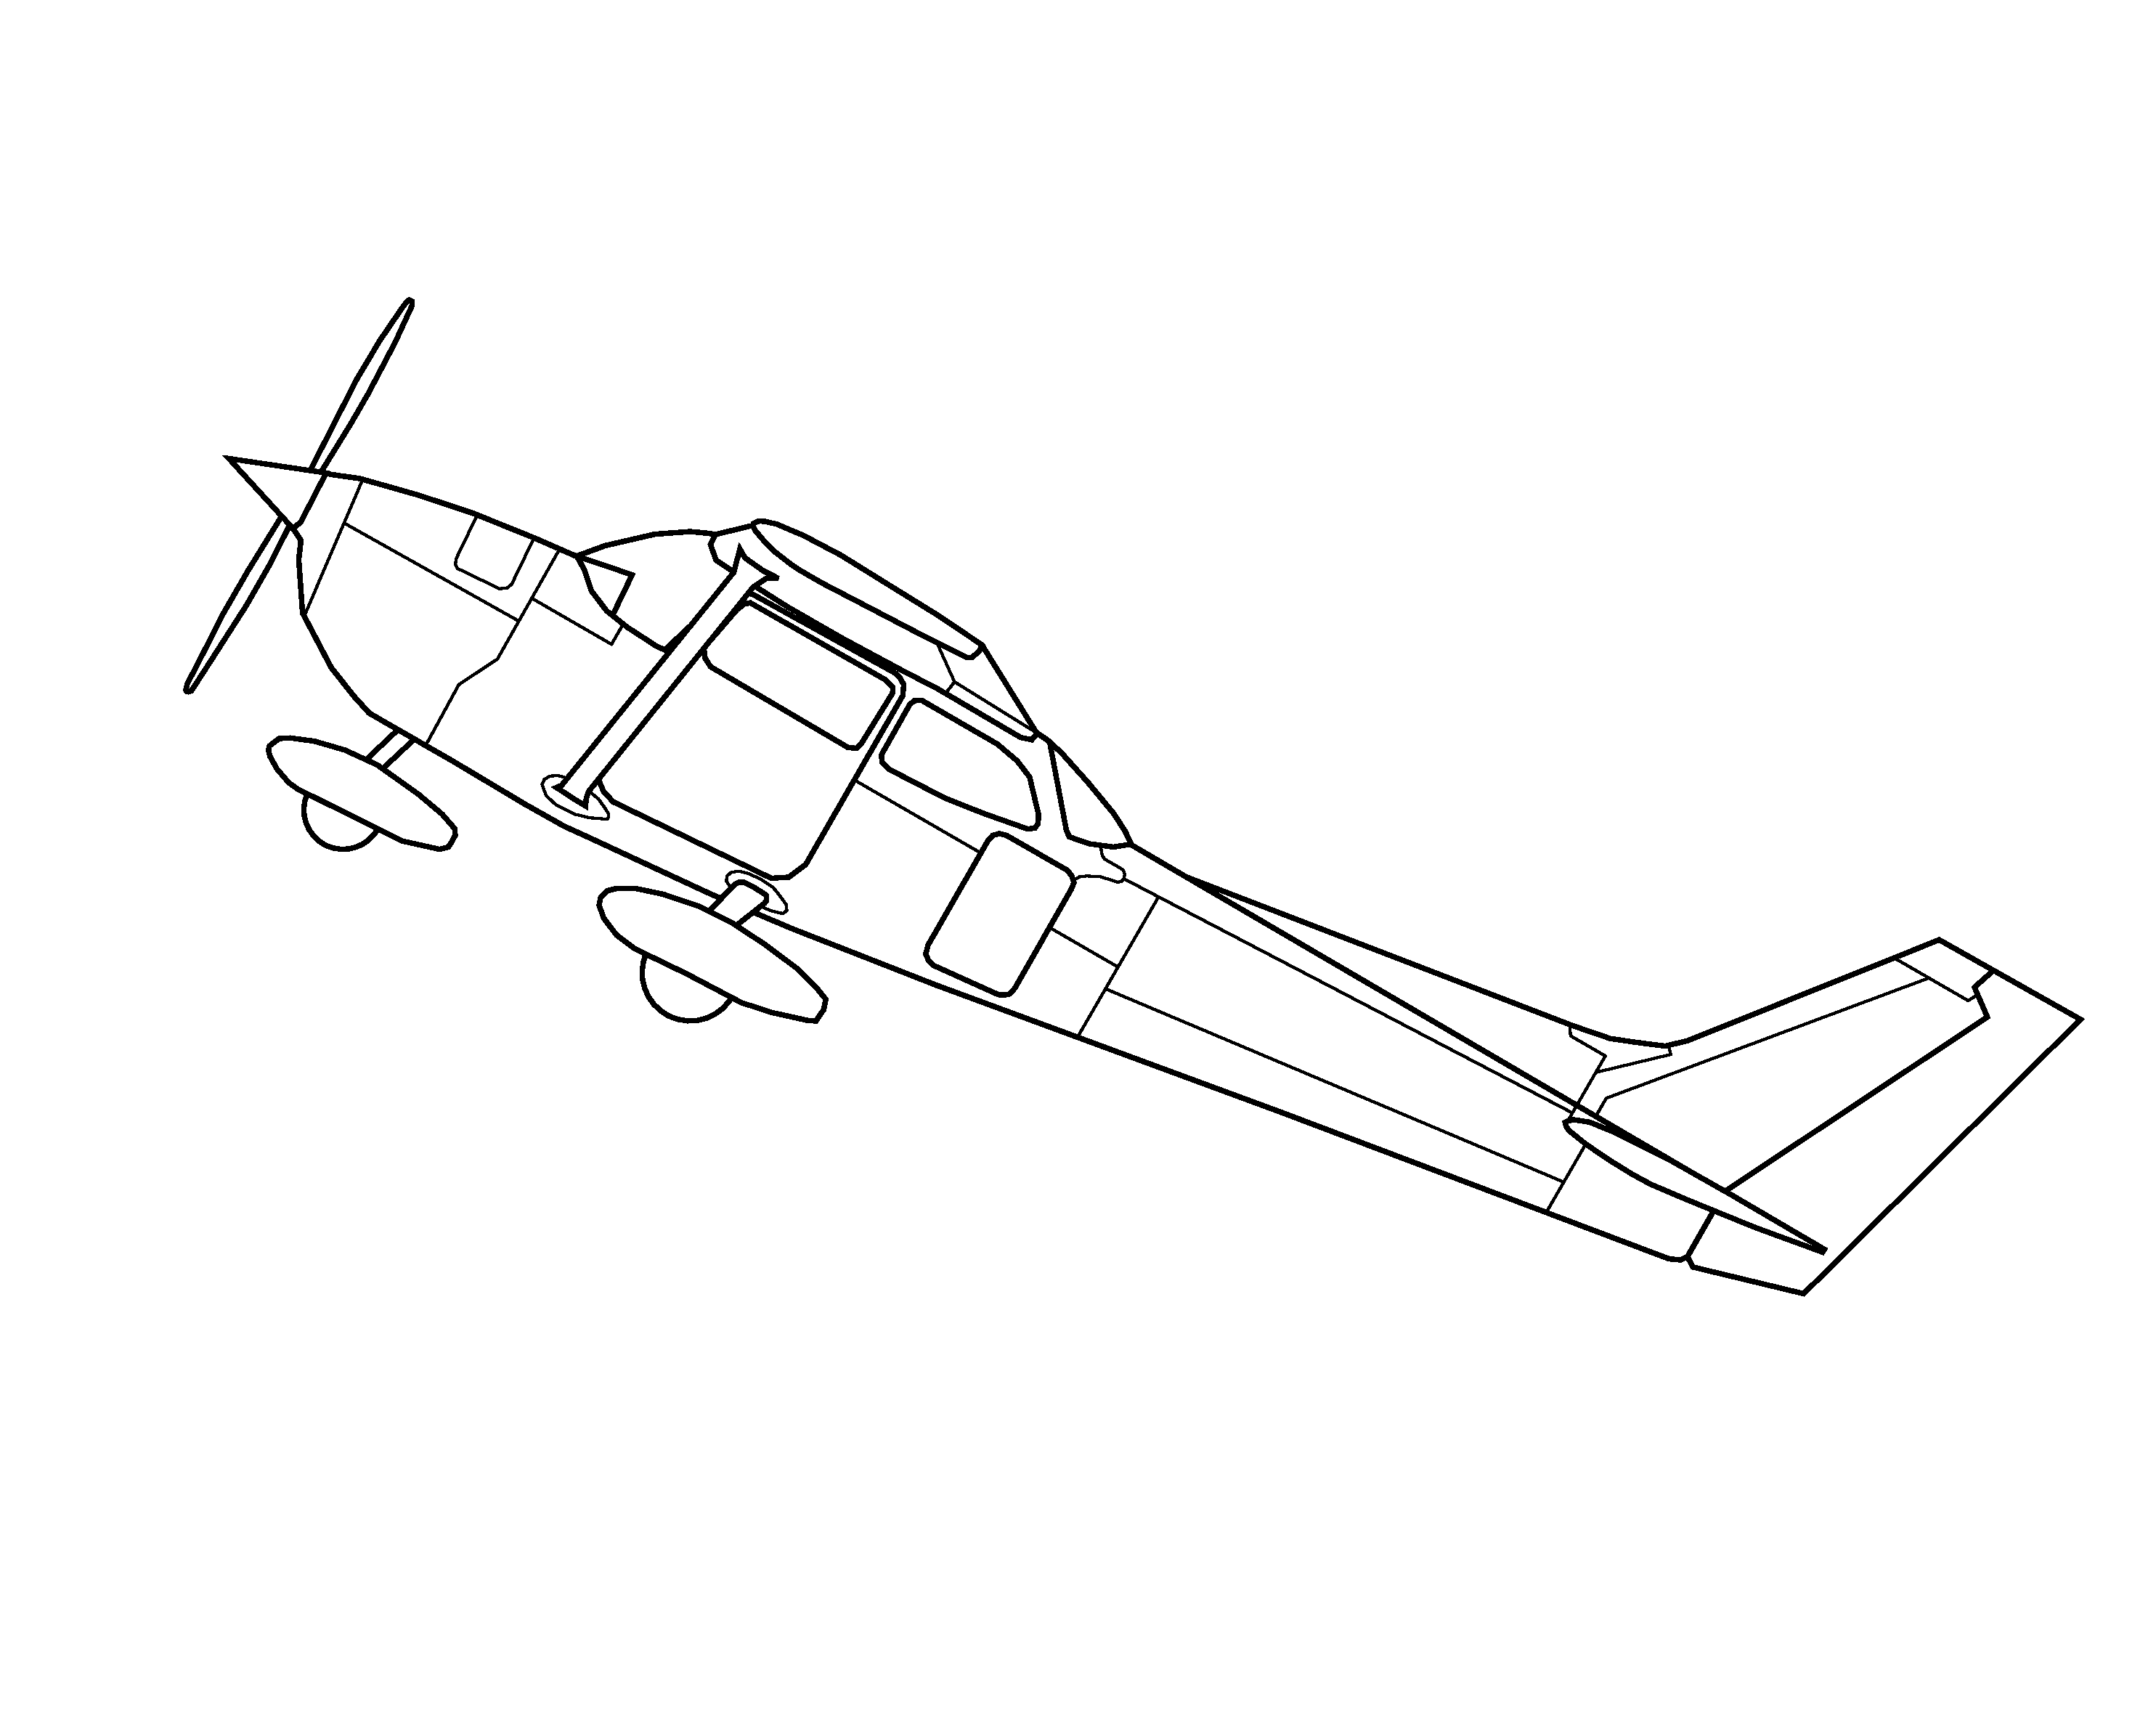
\includegraphics[width=0.6\textwidth]{../.images/airplane_pitch.eps}};

        % -----------
        % Parameters.
        % -----------
        
        % origin
        \pgfmathsetmacro{\Ox}{3.5}
        \pgfmathsetmacro{\Oy}{4.43}

        % pitch angle [deg]
        \pgfmathsetmacro{\pitchangle}{30}
        
        % axes length
        \pgfmathsetmacro{\axlen}{4}

        % arc radius
        \pgfmathsetmacro{\arcrad}{0.9*\axlen}

        % -----------
        % Body frame.
        % -----------
        
        % xb-axis endpoint
        \pgfmathsetmacro{\xbx}{\Ox-cos(\pitchangle)*\axlen}
        \pgfmathsetmacro{\xby}{\Oy+sin(\pitchangle)*\axlen}

        % zb-axis endpoint
        \pgfmathsetmacro{\zbx}{\Ox-sin(\pitchangle)*\axlen}
        \pgfmathsetmacro{\zby}{\Oy-cos(\pitchangle)*\axlen}

        % body axes
        \draw[line width=0.5mm](\Ox,\Oy)--(\xbx,\xby)node[pos=1.06]{$x_{b}$};
        \draw[line width=0.5mm](\Ox,\Oy)--(\zbx,\zby)node[pos=1.06]{$z_{b}$};

        % ------------
        % World frame.
        % ------------
        
        % xw-axis endpoint
        \pgfmathsetmacro{\xwx}{\Ox-\axlen}
        \pgfmathsetmacro{\xwy}{\Oy}

        % zw-axis endpoint
        \pgfmathsetmacro{\zwx}{\Ox}
        \pgfmathsetmacro{\zwy}{\Oy-\axlen}

        % world axes
        \draw[dotted,line width=0.5mm](\Ox,\Oy)--(\xwx,\xwy)node[pos=1.07]{$x_{w}$};
        \draw[dotted,line width=0.5mm](\Ox,\Oy)--(\zwx,\zwy)node[pos=1.06]{$z_{w}$};

        % ------------
        % Pitch angle.
        % ------------

        % arrow 1 starting point
        \pgfmathsetmacro{\arcx}{\Ox-\arcrad}
        \pgfmathsetmacro{\arcy}{\Oy}

        % arrow 1
        \draw[-mylatex',color_theme,thick](\arcx,\arcy)arc(180:150:\arcrad)node[midway,left]{$\theta_{\mathrm{world}\to\mathrm{body}}$};

        % arrow 2 starting point
        \pgfmathsetmacro{\arcx}{\Ox}
        \pgfmathsetmacro{\arcy}{\Oy-\arcrad}

        % arrow 2
        \draw[-mylatex',color_theme,thick](\arcx,\arcy)arc(270:240:\arcrad)node[midway,below]{$\theta_{\mathrm{world}\to\mathrm{body}}$};
        
    \end{tikzpicture}

\end{document}